\chapter{O que é a Ciência?\label{ciência:o:que:eh}}

Existem várias definições sobre o que é a ciência. Algumas questões sobre essa definição são apresentadas por \citep{fernandes_consideracoes_2021}, cujo texto está reproduzido a seguir. 

A figura \ref{fig:ciencia-filosofia}~ apresenta um mapa conceitual que trata da fundamentação do conceito de ciência e sua relação com a filosofia.
Veja o vídeo da aula de 20 de janeiro de 2022, para mais detalhes.

\begin{figure}[ht]
    \centering
    \caption{Conceitos fundamentais de ciência, e sua relação com a filosofia}
    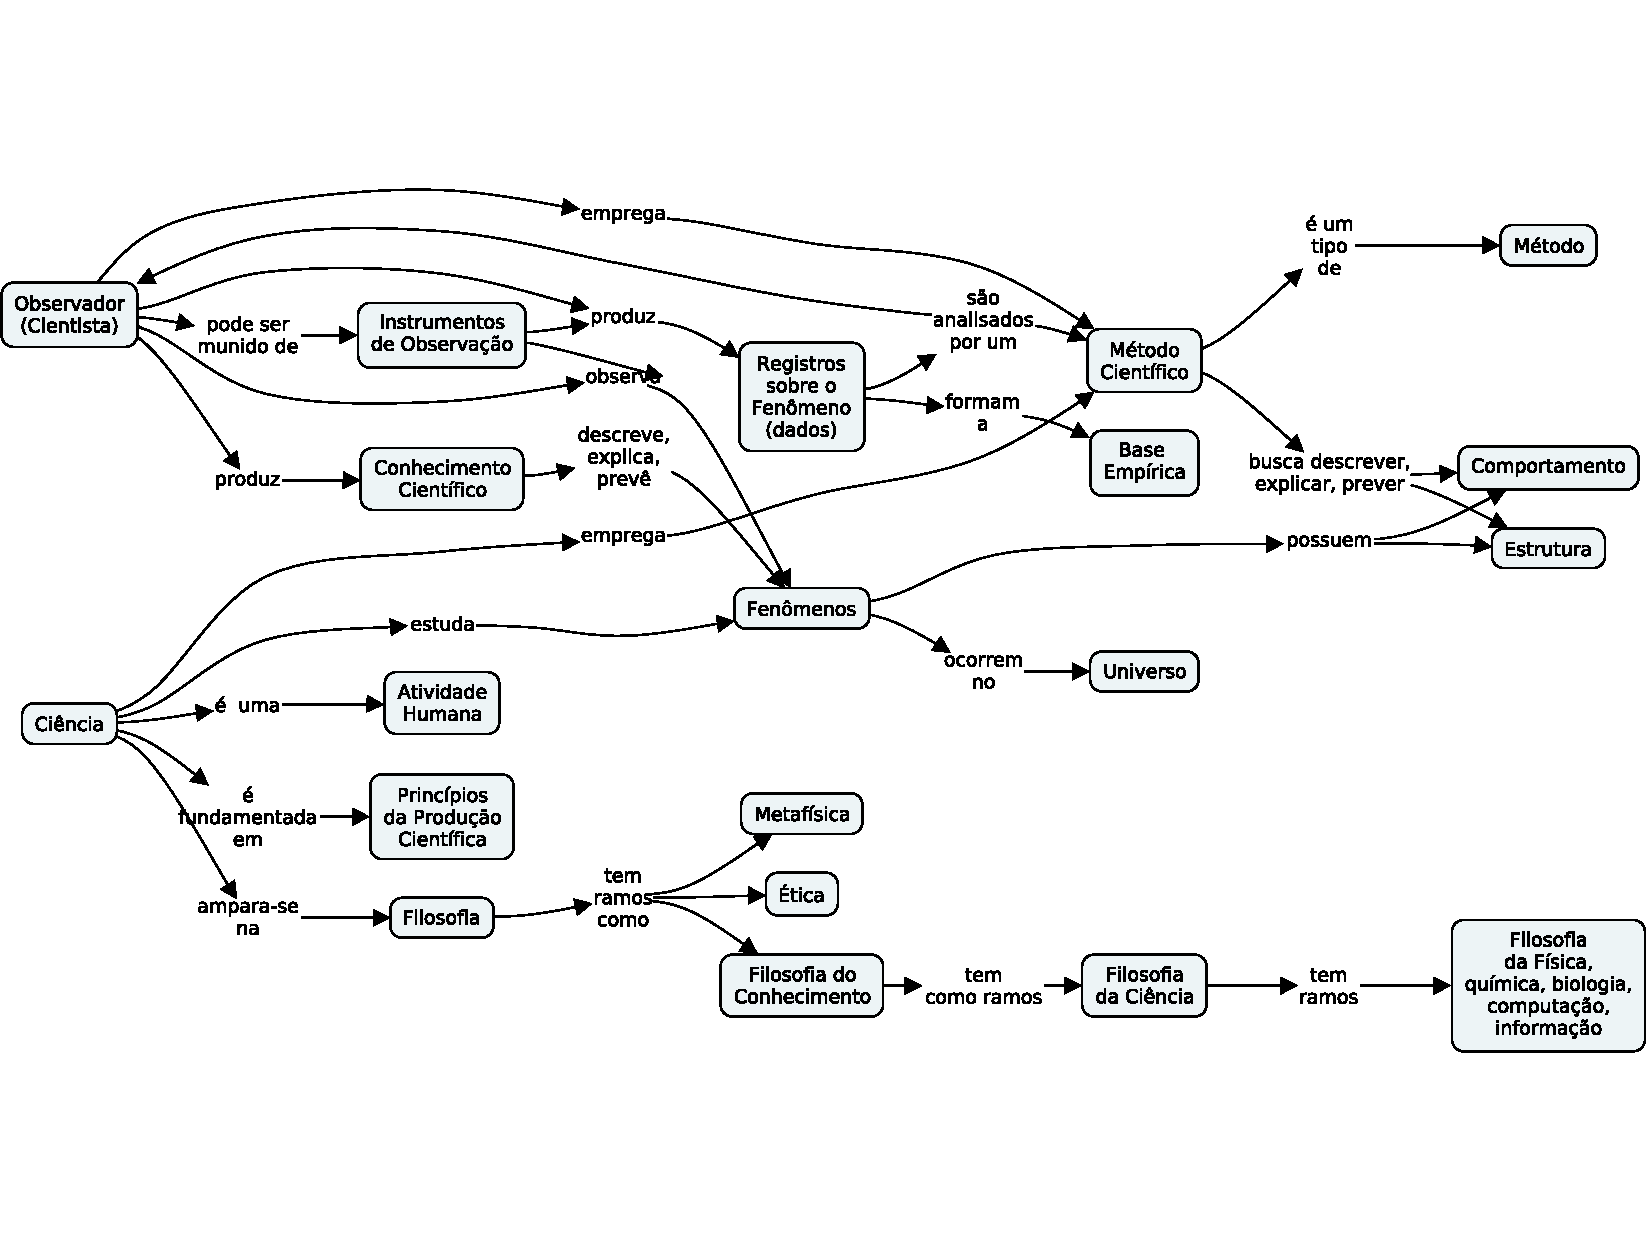
\includegraphics[page=1,angle=90,width=0.9\textwidth,height=0.9\textheight]{1-Introducao/aulas/Ciencia-e-Filosofia.pdf}
    \label{fig:ciencia-filosofia}
\end{figure}

A figura \ref{fig:desenv-sw-ciencia-filosofia} acrescenta à figura  \ref{fig:ciencia-filosofia}~ os conceitos que relacionam a natureza do desenvolvimento de software à  fundamentação do conceito de ciência e sua relação com a filosofia.
Veja o vídeo  da aula de 20 de janeiro de 2022, para mais detalhes.

\begin{figure}[ht]
    \centering
    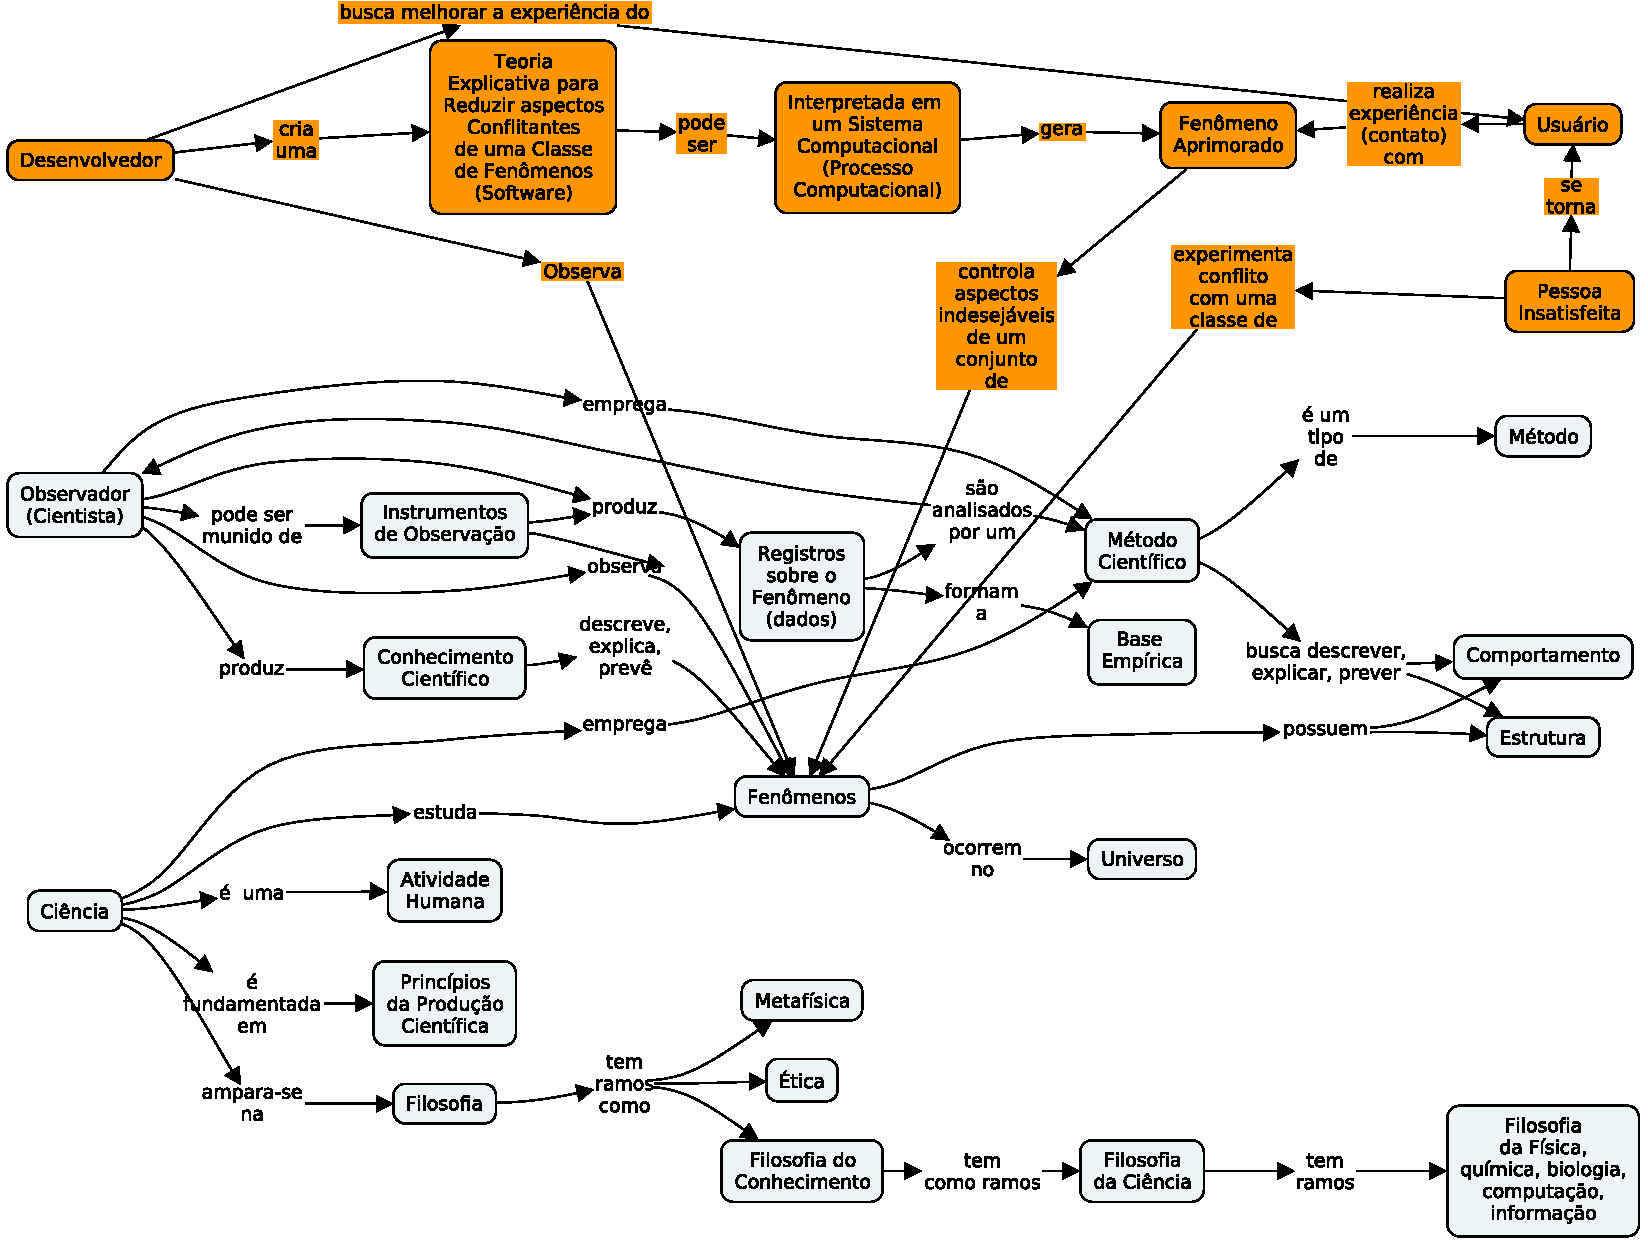
\includegraphics[page=1,angle=90,width=0.8\textwidth,height=0.9\textheight]{1-Introducao/aulas/Desenvolvimento-de-Software-Ciencia-e-Filosofia.pdf}
    \caption{Como a atividade do desenvolvimento de software se compara à atividade cientifica? Fonte: jhcf}
    \label{fig:desenv-sw-ciencia-filosofia}
\end{figure}

A figura \ref{fig:principios:ativ:cientifica}~ sumariza, em um mapa conceitual, os princípios da atividade científica e os relaciona com os princípios do desenvolvimento de software.
Veja o vídeo da aula de 20 de janeiro de 2022, para mais detalhes.

\begin{figure}[ht]
    \centering
    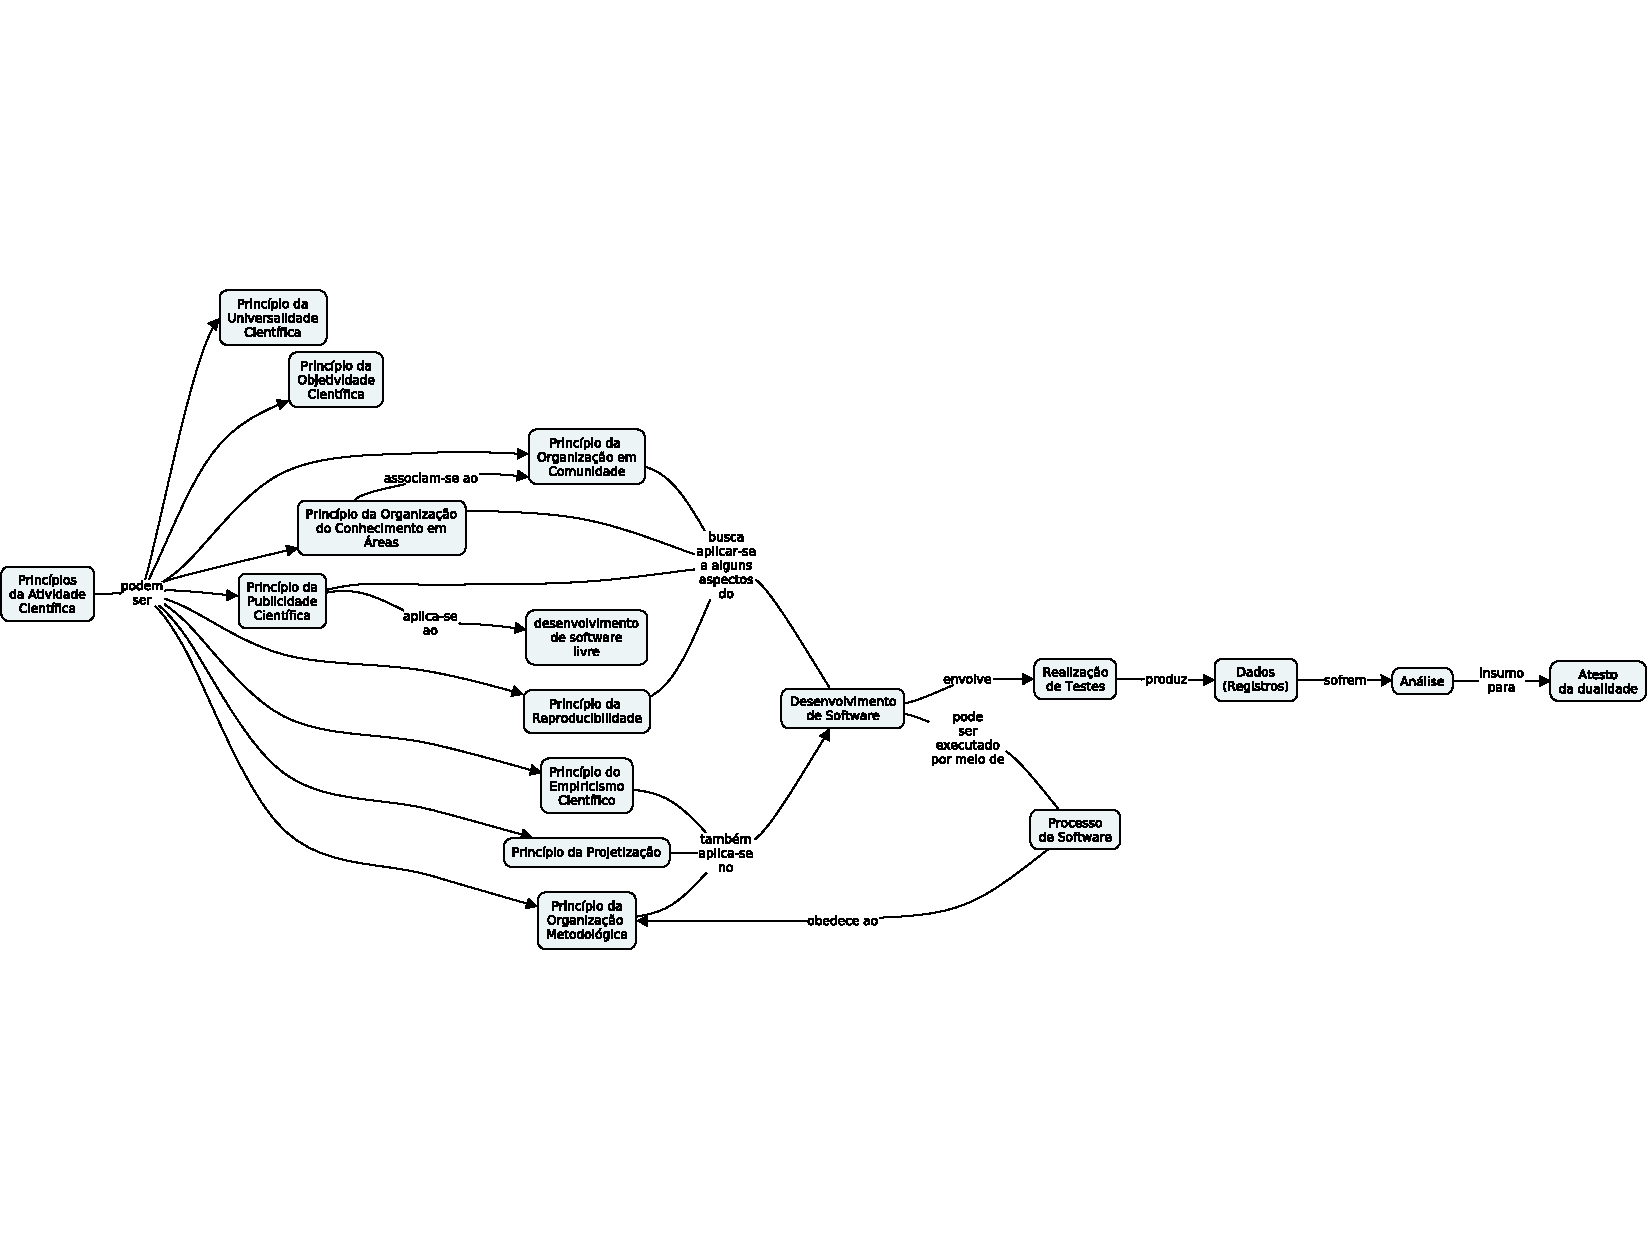
\includegraphics[page=1,angle=90,width=0.9\textwidth,height=0.9\textheight]{1-Introducao/aulas/Principios-da-atividade-cientifica.pdf}
    \caption{Quais os princípios da  atividade cientifica? como se relacionam com a atividade de desenvolvimento de software. Fonte: jhcf}
    \label{fig:principios:ativ:cientifica}
\end{figure}
